%#! platex thesis.tex
\documentclass[a4paper,12pt]{jreport}
\usepackage{jgraduate}          % 卒論・修論用スタイル

%% 索引作成
%\usepackage{makeidx}            
% dvipdfmxを使用しない場合はオプションを変更すること
\usepackage[dvipdfmx]{graphicx}
% 数字付きリストでラベルを使う
\usepackage{enumerate}          
% 数学記号など
\usepackage{amsmath}
\usepackage{amssymb}
\usepackage{amsthm}
% URLをいい感じにする
\usepackage{url}
\usepackage{cite}

%------------------------------
% 余白設定
%------------------------------
\usepackage[left=27mm,right=27mm,top=45mm,bottom=45mm,%
 headheight=5mm,headsep=10mm,%
 footskip=12mm%
 ]{geometry}

%------------------------------
% hyperref
%  日本語の文字コード設定が分からない人はコメントアウトすること.
%------------------------------
% PDF化したときにしおりが作成され,図表へのジャンプも可能となる.
\usepackage{atbegshi}
% Mac/Linuxの場合
%   ※Ubuntuの場合はEUC-UCS2を自分で入れないとダメ.
\AtBeginShipoutFirst{\special{pdf:tounicode EUC-UCS2}}
%% Winの場合
%\AtBeginShipoutFirst{\special{pdf:tounicode 90ms-RKSJ-UCS2}}
% 以下は共通
\usepackage[dvipdfm,a4paper,bookmarks,bookmarksnumbered,%
 bookmarksopen=false,pdfstartview={FitH},%
 bookmarkstype=toc,%
 setpagesize=false,%
 pdfauthor={九大 太郎},%
% setpagesize=false,% PDFのサイズがおかしい場合はこれを有効化
 pdftitle={俺の研究がこんなにすごいわけがない!}]{hyperref}

%----------------------------------------------------------------------
% 設定
%----------------------------------------------------------------------
% 目次の深さはsubsubsectionまで
\setcounter{tocdepth}{3}

% 基準となる図の幅
\newlength\figurewidth
\setlength{\figurewidth}{0.8\textwidth}
% 縦に並べた図の間の基準となるスペース
\newlength\figuresep
\setlength{\figuresep}{0.8\floatsep}

%----------------------------------------------------------------------
% 文書基本情報
%----------------------------------------------------------------------
% タイトル
\title{俺の研究が\\こんなに\\すごいわけがない!}

% 著者
\author{佐伯 優太}

% 所属
\university{九州大学}
\department{工学部}
\major{電気情報工学科}
%\university{九州大学大学院}
%\department{システム情報科学府}
%\major{情報知能工学専攻}

% 提出日(月までを書く)
\date{平成29年2月}

%% 書いている途中では以下のようにしておくと一部だけをタイプセットできる
%\includeonly{intro}

%======================================================================
% テキスト開始
%======================================================================
\begin{document}
% 表紙
\maketitle
% 表紙はページ番号を出力しない
\thispagestyle{empty}

%----------------------------------------------------------------------
% 概要
%----------------------------------------------------------------------
\begin{abstract}
%これは修論・卒論のテンプレートである.
テストテスト
テストaaaaaaaaaaaaaaaaaaaaaaaaaaaaaaaaaaaaaaaああああああああああああああああああ
\end{abstract}

%----------------------------------------------------------------------
% 目次のページ番号は1から
\setcounter{page}{0}
% 目次
\tableofcontents

% 本文のページ番号はアラビア数字
\pagenumbering{arabic}
 
%======================================================================
% 本文ここから
%======================================================================

% 章ごとのファイルを読み込む
% YaTeXなら各ファイルを読み込む行でC-c gでジャンプできる
%#! platex thesis.tex

%======================================================================
\chapter{はじめに}
\label{cha:intro}

%----------------------------------------------------------------------
\section{研究背景}
近年, ロボットの研究が注目されている. 中でも知能ロボットと呼ばれる人間の手足や指などに相当する運動機能のほかに, 視覚, 触覚, 聴覚などの感覚機能, および学習, 連想, 記憶, 推論などの思考機能を備えたロボットの研究がめざましい. 従来のロボットに比べ柔軟に対応することができる知能ロボットはより様々な場で活躍することが期待される. 例えば, 災害現場で人が立ち入るのが困難な場所へ向かい周囲の情報を提供したり, 被災者を発見したりといったことを行う災害救助ロボットや, 掃除や洗濯といったことを行う家庭用マルチサービスロボットなどが考えられる. これらのロボットではコンテキストと呼ばれる周囲の状況や, 内部の状態によって振る舞いを変えることが必要となる. 災害救助ロボットでは, 災害の状況によって移動方法を車輪からプロペラに変えたり, バッテリーの残量に応じて機能を制限したりする必要がある. また, 家庭用マルチサービスロボットでは, 周囲の湿度に合わせて掃除の方法を乾拭きから水拭きに変えたり, 屋内にいるか屋外にいるかで自己位置推定の方法を変更したりする必要がある. このようなコンテキストに応じて振る舞いを変えるようなロボットのことをコンテキストアウェアなロボットとする.\par
現在, ロボットの開発プラットフォームの標準化に対する研究が行われており, 中でもROS(ロボットオペレーティングシステム)と呼ばれるオープンソースのロボットソフトウェアが注目されている. ROSはメッセージベースのピアツーピア型のロボットミドルウェアであり, ROS上で開発されたソフトウェアモジュールは, 汎用性, 再利用性, 移植性に優れている.\par
コンテキストに依存する振る舞いを扱うための技術としてCOP(コンテキスト指向プログラミング)が提案されている. COPを用いることでコンテキストに依存する振る舞いの変更が可能になる.

%----------------------------------------------------------------------
\section{提案手法}
本論文ではロボットオペレーティングシステムにコンテキスト指向プログラミングを適用したContextROSを提案する.ContextROSでは,コンテキストの変更に応じた振る舞いの変更を可能にする.また,コンテキスト依存な振る舞いをまとめて記述することでコードの再利用性を高めている.



%----------------------------------------------------------------------
\section{論文の構成}
本論文の構成は以下の通りである.第2章ではコンテキストアウェアなロボットの開発に関する技術と既存研究を紹介する.第3章では提案手法についての説明を行う.第4章では提案手法のの評価を行う.最後に第5章でまとめとし,本研究の主たる成果と今後の課題について言及する.






% 以下はRefTeX用
%%% Local Variables:
%%% mode: yatex
%%% TeX-master: "bt_saeki"
%%% End:

%#! platex thesis.tex

%======================================================================
\chapter{おわりに}
\label{cha:conclu}

%----------------------------------------------------------------------
\section{本研究の主たる成果}
\label{sec:main-result}

何もねぇ...

本当にねぇ...

%----------------------------------------------------------------------
\section{今後の課題}
\label{sec:future}

課題なんてあろうか.
いや,あるわけがない.
全てが終わったのだから.


% 以下はRefTeX用
%%% Local Variables:
%%% mode: yatex
%%% TeX-master: "thesis"
%%% End:

%#! platex thesis.tex

%======================================================================
\chapter{はじめに}
\label{cha:intro}

%----------------------------------------------------------------------
\section{タイプセットの仕方}

TeXがインストールされていれば,
\begin{quote}
 \texttt{\$ make}
\end{quote}
を実行すればPDFファイルが生成される.
なお,\textbf{デフォルトの\texttt{Makefile}は\texttt{thesis.tex}の変更し
か参照しない}ため,必要であれば43行目にtexファイル名を追加する.
\texttt{make clean}するとPDFファイル以外で生成された中間ファイルの一部が
削除される.
また,\texttt{make cleanup}するとタイプセットに必要無いファイルはPDFファ
イルも含めて全て削除される.
Google Driveなどに登録する際は\texttt{make clean}してから登録すると良い.

\texttt{make}コマンドをインストールしていない場合は\texttt{platex}と
\texttt{pbibtex}(または\texttt{jbibtex})を適切な回数
(\texttt{platex}→\texttt{pbibtex}→\texttt{platex} 2回)実行し,
\texttt{.dvi}ファイルを生成する.
\begin{quote}
 \texttt{\$ platex thesis.tex}

 \texttt{\$ pbibtex thesis}

 \texttt{\$ platex thesis.tex}

 \texttt{\$ platex thesis.tex}
\end{quote}

その後\texttt{dvipdfmx}を使ってPDFを生成する.
\begin{quote}
 \texttt{\$ dvipdfmx thesis.dvi}
\end{quote}

なお,\texttt{make}では\texttt{pbibtex}も自動で実行するので,参考文献を
手で修正する場合は\texttt{.bbl}ファイルを\texttt{ref.tex}などの名前に変
更し,\texttt{Makefile}の
\begin{quote}
 \texttt{BIB = echo}
\end{quote}
を有効化すること.

\texttt{listings}パッケージを利用するとソースコード等の掲載が楽になる.
Macなどではデフォルトでインストールされているかと思うが,もしない場合は
\url{http://www.akita-nct.ac.jp/yamamoto/comp/latex/make_doc/source/source.html#listings}
あたりを参考にしてインストールする.
使い方は
\url{http://www.biwako.shiga-u.ac.jp/sensei/kumazawa/tex/listings.html}
あたりが参考になる.

なお,\texttt{make clean}すると中間ファイルを削除できる.
\texttt{make cleanup}とした場合には生成されたPDFファイルも削除される.

%----------------------------------------------------------------------
\section{このテンプレートの構成}

\begin{table}[bt]
 \centering
 \caption{テンプレートのファイル構成}
 \label{tab:files}
 \begin{tabular}{ll}\Hline
  各種\texttt{tex}ファイル & \texttt{thesis.tex}\\
  & \texttt{intro.tex}\\
  & \texttt{conclu.tex}\\
  & \texttt{ack.tex}\\
  & \texttt{public.tex}\\ \hline
  resume用ファイル & \texttt{resume.tex}\\
  & \texttt{resume.sty}\\ \hline
  修論・卒論スタイルファイル & \texttt{jgraduate.sty}\\ \hline
  信学会BiBTeXスタイルファイル & \texttt{sieicej.bst}\\ \hline
  ビルド設定 & \texttt{Makefile}\\ \hline
  サンプルbibファイル & \texttt{bib/}\\ \Hline
 \end{tabular}
\end{table}

\tablename~\ref{tab:files}に,このテンプレートに含まれているファイルを示
す.

章を追加する場合はファイルを追加する.
章ファイルの書き方は\texttt{conclu.tex}をマネすれば良い.
章ファイルを作成したら,\texttt{thesis.tex}に\texttt{\yen include}文を追
加する.

%----------------------------------------------------------------------
\section{基本情報の書き換え}

以下のファイルには名前や所属などの基本情報が書かれているため,全て書き換
えること.

\begin{enumerate}
 \item \texttt{thesis.tex}

       \texttt{pdfauthor},
       \texttt{pdftitle},
       \texttt{\yen title},
       \texttt{\yen author},
       \texttt{\yen university},
       \texttt{\yen department},
       \texttt{\yen major},
       \texttt{\yen date}
 \item \texttt{resume.tex}

       \texttt{\yen title},
       \texttt{\yen author},
       \texttt{\yen professor},
       \texttt{\yen date},
       \texttt{\yen time},
       \texttt{\yen location}
\end{enumerate}

%----------------------------------------------------------------------
\section{論文記述に関する基本的なルール}

\begin{enumerate}
 \item 主語を省略しないこと.
       省略していいのは2つの文が連続で同じ主語のときだけ.
       3つの文が連続して同じ主語になるのは好ましくないので,そのような場
       合には文を書き換えること.
 \item 1段落(1 paragraph)には1つの話題(topic)のみを記述する.
 \item 大事なことは最初に書く.
       例外は論文の一番最初の段落.
 \item 主語と述語を対応させる.
 \item 原則として1つの文は全角36文字折り返しで3行以内にする.
\end{enumerate}

%----------------------------------------------------------------------
\section{印刷に際する注意}

マージン(余白)が少ないと事務に提出する際に突き返される.
2015年度の規定では,上下の余白は30\,mm以上,左右の余白は25\,mm以上となっ
ている.

デフォルト設定では倍率100\,\%で印刷して大丈夫なようにしてあるが,環境に
よっては余白が小さくなるため必要に応じて\texttt{thesis.tex}内の
\texttt{geometry}パッケージのオプションを変更すること.

%----------------------------------------------------------------------
\section{Tips}

%--------------------------------------------------
\subsection{全般}

\begin{itemize}
 \item 情報系の論文は句読点として「,」「.」(全角)を用い,「〜だ」「〜
       である」調で記述する.
 \item 日本語本文中に括弧を使う場合は(このようにして)全角を使うこと.
       流儀にもよるが,基本的には中身が英語であっても全角を用いる(like
       this).
 \item 「1つ」などと数字を使った表記をする場合は半角の数字を使うこと.
 \item マイナスの数字で「-」と書くとハイフンになってしまうので,$-52$の
       ように数式モードを使うこと.
 \item \textbf{全角スペースは絶対に使用しない}こと!
 \item \texttt{\~}(半角チルダ)は改行されないスペースである.
       図表番号を記述する際などに使用する.
 \item コマンドなどは\texttt{make}などとして記述する.
 \item 単位や規格番号の前には\texttt{\yen ,}を入れると少しスペースが空い
       て見やすくなる.10\,mやIEEE\,802.15.4など.
 \item 図に英語を入れると福田先生に日本語にしろと言われるため,図は日本
       語で作成する.
       ただし,一般の論文では図は英語で書くことが望ましいため,日本語と
       英語の両方を作成しておく.
       \textbf{図の元ファイル(pptなど)も必ず残しておく}こと.
 \item 実験結果のグラフなどは,どのデータをどうやって描いたかが分かるよ
       うな記録を必ず残す.
       結果が間違っていたときに変更できないと捏造になるので注意すること.
 \item 英文における「.」(ピリオド)の使い方に注意.
       TeXでは
       \begin{enumerate}
        \item 大文字の後ろのピリオドでは終止符ではない.
        \item それ以外のピリオドは終止符.
       \end{enumerate}
       と判断されるため,「\texttt{GPS.}」のような場合にはピリオドが終止
       符でないと判断される.
       この場合は「\texttt{GPS\yen@.}」と書くこと.
       括弧は無視されるので,「\texttt{(GPS).}」のような場合も
       「\texttt{(GPS)\yen@.}」と書くこと.
       逆に,\texttt{Fig. 1}のような場合は「\texttt{Fig.\yen\ 1}」
       や「\texttt{Fig.\~{}1}」などと明示的にスペースを入れることで終止
       符でないことを示す.
\end{itemize}

%--------------------------------------------------
\subsection{図}

\begin{figure}[bt]
 \centering
 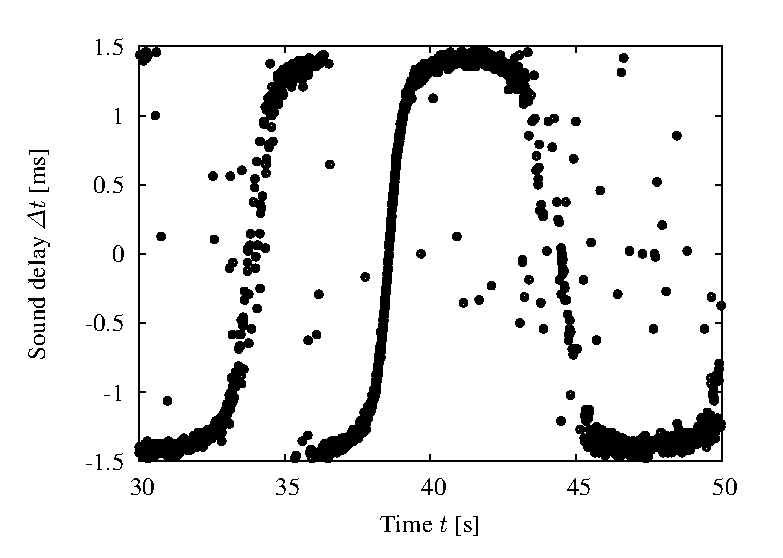
\includegraphics[width=\figurewidth]{img/test.eps}
 \caption{ダミーの図}
 \label{fig:test}
\end{figure}

図や表を入れる際の\texttt{figure},\texttt{table}環境のオプションでは
\texttt{[h]}は指定せず,\texttt{[bt]},\texttt{[btp]}などとする.

図を真ん中に表示させるには,\figurename~\ref{fig:test}のように
\texttt{\yen centering}を使う.
\texttt{center}環境を使うとムダなスペースが入ってしまう.
また,図や\texttt{section}を参照する場合は\texttt{\yen label}と
\texttt{\yen ref}を使う.

\begin{figure}[bt]
 \centering
 \begin{minipage}[b]{0.49\hsize}
  \centering
  \fbox{\rule{0pt}{2cm}\rule{0.4\figurewidth}{0pt}}\\
  (a)~ダミーの図1-1
 \end{minipage}
 \hfill
 \begin{minipage}[b]{0.49\hsize}
  \centering
  \fbox{\rule{0pt}{2cm}\rule{0.4\figurewidth}{0pt}}\\
  (b)~ダミーの図1-2
 \end{minipage}
 \caption{ダミーの図(横並べバージョン)}
 \label{fig_intro:dummy_fig1}
\end{figure}

\begin{figure}[bt]
 \centering
 \fbox{\rule{0.8\hsize}{0pt}\rule{0pt}{2cm}}\\
 (a)~ダミーの図2-1
 \vspace{\figuresep}

 \fbox{\rule{0.8\hsize}{0pt}\rule{0pt}{2cm}}\\
 (b)~ダミーの図2-2
 \caption{ダミーの図(縦積みバージョン)}
 \label{fig_intro:dummy_fig2}
\end{figure}

図を並べる時は\figurename~\ref{fig_intro:dummy_fig1}や
\figurename~\ref{fig_intro:dummy_fig2}のように書く.

%--------------------------------------------------
\subsection{表}

表の書き方は\tablename~\ref{tab:files}を参照のこと.
表に縦線を入れるとダサい感じになる.
区切りに使用するための太線として\texttt{\yen Hline}を用意しているので適
宜利用する.

%--------------------------------------------------
\subsection{リスト}

番号なしのリストは\texttt{itemize}環境を使う.
\begin{itemize}
 \item テスト1
 \item テスト2

       長い場合には段落を変えることもできるが,字下げはデフォルトでは無
       効になっている.
 \item テスト3
\end{itemize}

番号付きのリストは\texttt{enumerate}環境を使う.
\begin{enumerate}
 \item テスト1
 \item テスト2
\end{enumerate}

\texttt{enumerate}パッケージを使えば,番号付きリストにラベルを付けること
もできる.
\begin{enumerate}[(第1段階)]
 \item テスト段階
 \item テスト段階
\end{enumerate}

%--------------------------------------------------
\subsection{数式}

インラインの数式は$y=x^2+x+2$のように\texttt{\$}で囲うことで記述できる.
1行を使う数式は\texttt{equation}環境を使う.
\begin{equation}
 f(x) = \int_0^{2\pi}\frac{\sin x}{x}\,dx
  \label{eq:test_eq}
\end{equation}
数式を参照する場合は,式~(\ref{eq:test_eq})のように\texttt{\yen label},
\texttt{\yen ref}を用いる.

数式番号を付けたくない場合は環境名に\texttt{*}を付ける.
\begin{equation*}
 f(x) = \int_0^{2\pi}\frac{\sin x}{x}\,dx
\end{equation*}


複数行の数式は\texttt{align}環境を使用する.
\texttt{\&}は位置を揃えるためのマークであり,出力はされない.
数式番号を出力したくない行には\texttt{\yen nonumber}を付ける.
\begin{align}
 f(x) &= \int_0^{2\pi}\frac{\sin x}{x}\,dx \nonumber\\
 g(x) &= \int_0^{2\pi}\frac{\cos x}{x}\,dx
\end{align}

括弧を使う場合は大きさが自動的に変わるように\texttt{\yen left}などと組み
合わせて使用する.
\begin{align*}
 S &= \sum_k \delta_{ij}[k] \\
 U &= \sum_k \left( \zeta[k] + 3\sum_{l=0}^k \delta_{ij}[l] \right)
\end{align*}

数式中で複数文字から成る変数を表現する際は,ときと場合によってスペースが
広がりすぎるのを防ぐため\texttt{\yen mathrm}や\texttt{\yen mathit}でまと
める.

\begin{equation*}
 \left\{
 \begin{array}{rcl}
  P_{t1} - L_\mathit{loss} &=& \mathrm{RSS}_1\\
  P_{t2} - L_\mathit{loss} &=& \mathrm{RSS}_2\\
  &\vdots&
 \end{array}
 \right.
\end{equation*}

%--------------------------------------------------
\subsection{引用}

\texttt{.bib}ファイルを作成し,本文中で\texttt{\yen cite}を使って参照す
る~\cite{wu13:will_pds}.
その上で\texttt{pbibtex}または\texttt{jbibtex}を使って\texttt{.bbl}ファ
イルを生成する.
一度に複数書くこともでき
る~\cite{scholten08:cmc_psp,nakauchi05:intelli_kitchen%
,yang12:locate_finger}.


% 以下はRefTeX用
%%% Local Variables:
%%% mode: yatex
%%% TeX-master: "thesis"
%%% End:

% 謝辞
%#! platex thesis.tex
%======================================================================
% 謝辞
%======================================================================
\acknowledgment

あり〜がと〜\\
さよ〜なら〜\\
きょ〜しつ〜\\
しかられたこと〜さえ〜\\
あ〜たた〜か〜い〜

\newpage

謝辞が2ページになったときのテスト.


%----------------------------------------------------------------------
% 参考文献
%----------------------------------------------------------------------
\bibliographystyle{sieicej}
\bibliography{bib/IEEEfull,bib/mystr_IEEEfull,bib/my,bib/pub}
% 書き終えたら,↑の2行をコメントアウトして,BibTeXが生成したthesis.bbl
% をref.texという名前に変更して
% ↓を有効化するとよい.必要があれば手動で修正する.
%\include{ref}

%----------------------------------------------------------------------
% 発表文献
%----------------------------------------------------------------------
%#!platex thesis.tex
%======================================================================
% Publications
%======================================================================
\publications

% 数が少なければ項目に分ける必要はないです.
% section*の区切りを削除して下さい.

%----------------------------------------------------------------------
\section*{学術雑誌等(査読あり) }
\begin{publication}{99}
\bibitem{mlab/ishida11:wake-up_ieice_trans}
石田繁巳,瀧口貴啓,猿渡俊介,南\hskip1zw正輝,森川博之,
``ブルームフィルタを用いたウェイクアップ型通信システム,\<''
電子情報通信学会論文誌B: 通信,
vol.J94-B,no.10,pp.1397--1407,Oct.\ 2011.

\end{publication}

%----------------------------------------------------------------------
%\section*{学術雑誌等または商業誌における解説,総説}
%\begin{publication}{P99}
%\end{publication}

%----------------------------------------------------------------------
\section*{国際会議における発表}
\subsection*{口頭発表(査読あり)}
\begin{publication}{99}
\bibitem{mlab/takiguchi09:wakeup_greencomm}
T. Takiguchi, S. Saruwatari, T. Morito, S. Ishida, M. Minami, and H. Morikawa,
``A novel wireless wake-up mechanism for energy-efficient ubiquitous
  networks,''
Proceedings of the {IEEE} Workshop on Green Communications (GreenComm),
pp.1--5, June 2009.

\bibitem{mlab/ishida10:apsitt}
S. Ishida, T. Takiguchi, S. Saruwatari, M. Minami, and H. Morikawa,
``Evaluation of a wake-up wireless module with bloom-filter-based {ID}
  matching,''
Proceedings of Asia-Pacific Symposium on Information and Telecommunication
  Technologies (APSITT),
pp.1--6, June 2010.

\end{publication}

%--------------------------------------------------
\subsection*{ポスター,デモ発表(査読あり)}
\begin{publication}{99}
\bibitem{mlab/ishida06:percom_demo}
S. Ishida, M. Minami, Y. Nishizawa, T. Morito, Y. Moriyama, H. Morikawa, and T.
  Aoyama,
``Three devices for tackling practical problems in pervasive computing,''
IEEE International Conference on Pervasive Computing and Communications
  (PerCom), Demo,
p.1,
D8, March 2006.

\bibitem{mlab/ishida10:iot}
S. Ishida, T. Takiguchi, S. Saruwatari, M. Minami, and H. Morikawa,
``Implementation of bloom-filter-based {ID} matching for wake-up wireless
  communication,''
Internet of Things 2010 Conference (IoT 2010), poster, Dec.\ 2010.

\end{publication}

%----------------------------------------------------------------------
\section*{研究会}
\begin{publication}{99}
\bibitem{mlab/Ishida08:wakeup_in}
石田繁巳,鈴木\hskip1zw誠,森戸\hskip1zw貴,森川博之,
``低受信待機電力無線通信のための多段ウェイクアップ機構,\<''
電子情報通信学会技術報告,
pp.355--360,
情報ネットワーク研究会(IN2007-218),March 2008.

\bibitem{mlab/takiguchi10:bloom_rcs}
瀧口貴啓,石田繁巳,猿渡俊介,南\hskip1zw正輝,森川博之,
``ブルームフィルタを用いたウェイクアップ型無線通信システムの消費電力評価,\<''
電子情報通信学会技術報告,
pp.269--274,
無線通信システム研究会(RCS2009-254),Jan.\ 2010.

\bibitem{mlab/takiguchi11:wakeup_in}
瀧口貴啓,石田繁巳,岸\hskip1zw孝彦,丹羽栄二,見並一明,猿渡俊介,森川博之,
``ウェイクアップ型無線通信におけるビット不一致許容{ID}マッチング,\<''
電子情報通信学会技術報告,
pp.193--198,
情報ネットワーク研究会(IN2010-176),March 2011.

\end{publication}

%----------------------------------------------------------------------
\section*{全国大会}
\begin{publication}{99}
\bibitem{mlab/matsui07:wake-up_st}
松井壮介,石田繁巳,鈴木\hskip1zw誠,猿渡俊介,森川博之,
``実験的アプローチによるシングルホップ通信とマルチホップ通信の消費電力の比較,%
\<''
電子情報通信学会総合大会,
p.1,
A-21-22,March 2007.

\bibitem{mlab/ishida07:wake-up_st}
石田繁巳,猿渡俊介,鈴木\hskip1zw誠,森川博之,
``サービス発見のためのゼロ受信待機電力無線システムの設計,\<''
電子情報通信学会総合大会,
p.1,
B-7-202,March 2007.

\bibitem{mlab/ishida08:wake-up_st}
石田繁巳,鈴木\hskip1zw誠,森戸\hskip1zw貴,森川博之,
``低受信待機電力無線通信のための階層型ウェイクアップ機構,\<''
電子情報通信学会総合大会,
p.1,
B-5-112,March 2008.

\bibitem{mlab/ishida10:wake-up_imple}
石田繁巳,瀧口貴啓,猿渡俊介,南\hskip1zw正輝,森川博之,
``ウェイクアップ型無線通信のためのグループ指定可能{ID}マッチング機構の実装,\<%
''
電子情報通信学会ソサイエティ大会,
p.1,
B-5-140,Sept.\ 2010.

\bibitem{mlab/ishida11:wake-up_sogo}
石田繁巳,瀧口貴啓,猿渡俊介,森川博之,
``ブルームフィルタを用いたウェイクアップ型無線通信システムにおける{ID}長の影響%
,\<''
電子情報通信学会総合大会,
p.1,
B-5-146,March 2011.

\bibitem{mlab/takiguchi11:wake-up_sogo}
瀧口貴啓,石田繁巳,岸\hskip1zw孝彦,丹羽栄二,見並一明,猿渡俊介,森川博之,
``車両内ウェイクアップ型無線通信における数個のビット不一致許容{ID}マッチング,%
\<''
電子情報通信学会総合大会,
p.1,
B-5-145,March 2011.

\bibitem{mlab/okamura11:sogo}
岡村悠貴,鈴木\hskip1zw誠,石田繁巳,今泉英明,関谷勇司,森川博之,
``非同期光パケットリングにおける高帯域利用効率パケット選択方式,\<''
電子情報通信学会総合大会,
p.1,
B-10-96,March 2011.

\bibitem{mlab/ishida11:mixer_sotai}
石田繁巳,鈴木\hskip1zw誠,森川博之,
``サブスレッショルド特性を利用するウェイクアップ受信機用ミキサの初期的検討,\<%
''
電子情報通信学会ソサイエティ大会,
p.1,
C-12-16,Sept.\ 2011.

\bibitem{mlab/kim11:spectrum_sotai}
金\hskip1zw昊俊,長縄潤一,石田繁巳,鈴木\hskip1zw誠,森川博之,
``可変{RBW}を用いた周波数占有率の測定精度の初期的評価,\<''
電子情報通信学会ソサイエティ大会,
p.1,
B-17-8,Sept.\ 2011.

\bibitem{mlab/nakamura11:co2_visual_sotai}
中村元紀,中村隆幸,荒川\hskip1zw豊,東島由佳,柏木啓一郎,森\hskip1zw皓平,松%
村\hskip1zw一,石田繁巳,猿渡俊介,翁長\hskip1zw久,森川博之,
``{uTupleSpace}を利用した$\mathrm{CO_2}$排出量可視化の実証実験,\<''
電子情報通信学会ソサイエティ大会,
p.1,
B-19-21,Sept.\ 2011.

\bibitem{mlab/nakajima12:spfc_sogo}
中嶋毅彰,米川\hskip1zw慧,石田繁巳,鈴木\hskip1zw誠,森川博之,
``多様なサービス電力の発見・割当て・制御機構,\<''
電子情報通信学会総合大会,
p.1,
BS-4-2,March 2012.

\end{publication}

%----------------------------------------------------------------------
\section*{その他の学会等}
\begin{publication}{99}
\bibitem{mlab/ishida09:inria}
S. Ishida,
``Wake-up wireless communication system for energy-efficient ubiquitous
  network,''
INRIA-TODAI Workshop (GCOE-INRIA Workshop), oral presentation, Dec.\ 2009.

\bibitem{mlab/ishida10:hakone_mct}
S. Ishida,
``Design of a zero-power-listening wireless system for service discovery,''
1st International Workshop on Microwatt Communication Technology, Jan.\ 2010.

\bibitem{mlab/ishida10:google_workshop}
S. Ishida,
``Wake-up wireless communication system,''
Tech Talks and Mix at Google Tokyo, oral presentation, Dec.\ 2010.

\bibitem{mlab/kak-t10:health_poster}
角田\hskip1zw仁,中嶋毅彰,石田繁巳,猿渡俊介,森川博之,
``社会実装に向けたヘルスケア情報共有基盤,\<''
第5回人間情報学会講演会,ポスター,Dec.\ 2010.

\end{publication}


\end{document}
